\begin{problem}{Upside down primes}{standard input}{standard output}{primes}

Last night, I must have dropped my alarm clock. When the alarm went off in the morning, it showed
51:80 instead of 08:15. This made me realize that if you rotate a seven segment display like it is
used in digital clocks by 180 degrees, some numbers still are numbers after turning them upside
down.

\begin{center}
  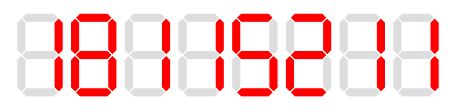
\includegraphics[scale=0.5]{./texts/src/b1.png}\\
  Figure B-1: Prime number 18115211 on a seven segment display (see third sample).\\
  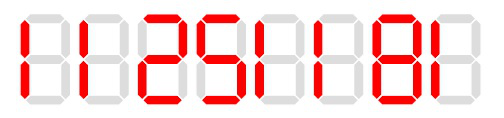
\includegraphics[scale=0.5]{./texts/src/b2.png}\\
  Figure B-2: 18115211 turned upside down (i.e. rotated by 180 degrees) gives 11251181, whichis not
              prime.
\end{center}

As you can see,\\
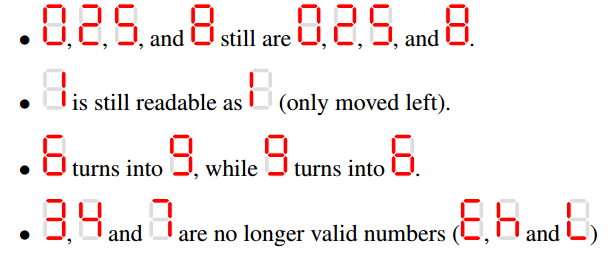
\includegraphics[scale=0.5]{./texts/src/b3.png}\\

My favourite numbers are primes, of course. Your job is to check whether a number
\textbf{is a prime} and \textbf{still a prime} when turned upside down.\\

\InputFile

One line with the integer $N$ in question $(1 \leq N \leq 10^{16})$. $N$ will not have leading
zeros.

\OutputFile
Print one line of output containing ``yes'' if the number \textbf{is a prime} and
\textbf{still a prime} if turned upside down, ``no'' otherwise.\\

\Example

\begin{example}
\exmp{
151
}{
yes
}%
\exmp{
23
}{
no
}%
\exmp{
18115211
}{
no
}%
\end{example}

\end{problem}
